\section{Basisløsninger}

%Jeg har endnu ikke fået gennemgået beviserne til de to sætninger ordentligt. de er bare stjålet fra jer andre.

Basisløsninger danner grundlaget for udregningen af den optimale løsning, hvilket beskrives og anvendes i Kapitel \ref{afsnit:simplex}. For at kunne beskrive netop basisløsninger er det nødvendigt først at introducere definitionen for \textbf{aktive betingelser}.%Ved ikke: Skal vi også bruge fed når ord introduceres i bindende tekst?

\begin{defn}[Aktive betingelser]
En betingelse siges at være \textbf{aktiv} for en givet løsningsvektor $\vec{x}$, hvis det gælder, at\\ $\vec{a}_i^T \vec{x}^* = b_i$.
\label{def:aktiv}
\end{defn}

Generelt bliver aktive betingelser brugt, da de for uligheder repræsenterer en grænse for de mulige løsninger i en given retning, mens de for ligheder blot beskriver, at betingelsen er opfyldt.
Yderligere anvendes skæringen mellem disse aktive betingelser, da den optimale løsning for lineære programmeringsproblemer findes i netop disse skæringer. Hvorfor dette netop er tilfældet bliver begrundet i Afsnit \ref{sec:eksistens}.

\begin{stn}[Lineært uafhængige rækker]
Lad $\vec{x}^* \in \mathds{R}^n$ og $I = \{i | \vec{a_i}^T \vec{x}^* = b_i\}$ være mængden af indekser for aktive betingelser. Da er følgende ækvivalent
\begin{enumerate}[label=(\alph*)]
\item Mængden $R_a =\{\vec{a_i}| i\in I\}$ indeholder vektorer, hvoraf $n$ af dem er lineært uafhængige.
\item Spannet $span(R_a) = \mathds{R}^n$.
\item Ligningssystemet $\vec{a_i}^T \vec{x}^* = b_i$, for $i \in I$ har en unik løsning.
\end{enumerate}
\label{stn:uniklosning}
\end{stn} %Ved ikke: Bør det siges at $\vec{a_i}$ repræcentere en række, eller er det underforstået i rapporten da den altid gør det?

\begin{proof}
	(a) <=> (b): Antag at der i $R_a$ er $n$ lineært uafhængige vektorer. Da der er $n$ lineært uafhængige vektorer må dimensionen af spannet af $R_a$ være $n$. Da $dim(span(R_a))=dim(\mathds{R}^n)=n$ og da $R_a \subseteq \mathds{R}^n$ må det følge af Sætning \ref{stn:dimunderrum} at $span(R_a)=\mathds{R}^n$. Tilsvarende gælder det at hvis $span(R_a)=\mathds{R}^n$, må det gælde at $dim(span(R_a))=dim(\mathds{R}^n)=n$. Da vil kardinaliteten af en basis for $R_a$ nødvendigvis være $n$, hvorved $R_a$ skal indeholde $n$ lineært uafhængige vektorer.


(a) <=> (c): Antag at $span(R_a)=\mathds{R}^n$. Antag nu for modstrid at der findes to løsninger, $\vec{x}_a$ og $\vec{x}_b$ som opfylder $\vec{a}_i\vec{x}=\vec{b}$ for alle $i \in I$. 
Da vil det for alle $i \in I$ gælde at $\vec{a}_i^T\vec{x}_a=\vec{b}$ og at $\vec{a}_i^T\vec{x}_b=\vec{b}$, hvorved $\vec{a}_i^T\vec{d}=\vec{0}$, hvor $\vec{d}=\vec{x}_a-\vec{x}_b$. 
Vektoren $\vec{d}$ vil da være orthogonal på alle $\vec{a}_i$ for $i \in I$ og kan derfor ikke være en lineær kombination af disse. Herved kan $R_a$ ikke udspænde hele $\mathds{R}^n$, da $\vec{d} \in \mathds{R}^n$ men $\vec{d} \notin span(R_a)$.
Tilsvarende antages det nu at der kun er en unik løsning til ligningssystemet. For modstrid antages det at $R_a$ ikke udspænder hele $\mathds{R}^n$ Der kan derved vælges en vektor $\vec{d}$ som er orthogonal til $span(R_a)$ hvorved $\vec{a}_i^T(\vec{x}+\vec{d})=\vec{b}$. derved er $\vec{x}$ ikke en unik løsning og der er opstået modstrid.
\end{proof}
	
	
	
	%Da er disse vektorer en basis for det underrum af $\mathds{R}^n$, som de udspænder. Da $dim(\mathds{R}^n)=dim(R_a)=n$ medfører det af sætning [4.59] at $span(R_a)=\mathds{R}^n$. Tilsvarende gælder det at hvis $span(R_a)=\mathds{R}^n$, må det gælde at $dim(span(R_a))=dim(\mathds{R}^n)=n$. Da vil kardinaliteten af en basis for $R_a$ nødvendigvis være $n$, hvorved $R_a$ skal indeholde $n$ lineært uafhængige vektorer.



%\begin{proof}
%(a) => (c): Lad $A$ være en $n \times n$ matrix bestående af rækkerne $\vec{a_i} \in R_a$, og antag at alle $\vec{a_i}$ er lineært uafhængige. 
%Antag nu for modstrid at ligningssystemet $A\vec{x} = \vec{b}$, hvor $\vec{b}$ har indgangende $b_i$ for $i \in I$, har to løsninger. 
%Da vil $A \vec{x} = \vec{b}$ og $A \vec{y} = \vec{b}$ hvorfor $A(\vec{x}-\vec{y}) = \vec{0}$.
%Derfor må søjlerne enten være lineært afhængige, eller $(\vec{x}-\vec{y})= \vec{0}$.
%Da der er $n$ lineært uafhængige rækker i $A$ må $rank(A) = n$, hvorfor alle søjler er lineært uafhængige, da $A$ er en $n \times n$ matrix.
%Det medfører at $\vec{x}-\vec{y} = \vec{0}$, hvorfor det kan konkluderes at løsningen til ligningssystemet er unikt da $ \vec{x}=\vec{y}$, og der derved er bevist modstrid.
%\\(c) => (a): Antag at der er en unik løsning til $A\vec{x} =\vec{b}$. Det medfører at der er en pivotindgang i hver række hvorved: $rank(A) = n$. hvorfor alle rækker må være lineært uafhængige, da $A$ er en $n \times n$ matrice. % s. 78-79 LinAlg
%\\ (a) => (b): Da $R_a$ består af $n$ linært uafhængige $n$-dimentionelle vektorer, må $R_a$ udgøre en base for $\mathds{R}^n$, hvorfor $span(R_a) = \mathds{R}^n$.
%\\ (b) => (a): Antag for modstrid, at vektorene i $R_a$ ikke er lineært uafhængige, da vil der eksistere en vektor $\vec{a}_i \in R_a$ som er en linear kombination af de andre vektorer, der må derfor eksistere en vektor $A\vec{x} = \vec{0}$, hvor $\vec{x} \neq \vec{0}$.
%Da det kun kan lade sig gøre hvis $\vec{x}$ er ortogonal med alle rækker i $A$, kan $\vec{x}$ ikke være en linear kombination af vektorene i $R_a$.
%Hvorfor at $\vec{x} \notin span(R_a)$.
%Derfor kan $span(R_a) \neq \mathds{R}^n$, hvorfor der er opstået modstrid.
%\end{proof}

\begin{defn}[Basisløsning]
Lad $P$ være et polyeder dannet af lineære bibetingelser, og lad $\vec{x}^*\in \mathds{R}^n$. Da er $\vec{x}^*$ en \textbf{basisløsning} hvis
\begin{enumerate}[label=(\alph*)]
\item Alle lighedskrav er aktive
\item Der er $n$ lineært uafhængige aktive betingelser
\end{enumerate}
og en \textbf{mulig basisløsning} hvis
\begin{enumerate}[label=(\alph*)]
\setcounter{enumi}{2}
\item $\vec{x}^*$ opfylder alle krav.
\end{enumerate}
\label{def:basislosning}
\end{defn}

Enhver bibetingelse udspænder et rum, for hvilket betingelsen er opfyldt. Skæringen, af de aktive betingelser, danner derved et rum, som er fællesmængden, af betingelsernes udspændte rum. Skæringen, af en mængde af aktive betingelser, svarer derved til den mulige mængde af disse betingelser. Dog gælder det for basisløsninger pr. Definition \ref{def:basislosning}, at der for en basisløsning $\vec{x}$ skal være $n$ lineært uafhængige aktive betingelser, hvorved en basisløsningen er en unik vektor, hvilket er bevist igennem Sætning \ref{stn:uniklosning}. %Ved ikke, er en vektor og et punkt det samme?

\begin{kor}[Endelig mængde af basisløsninger]
Givet en endelig mængde af bibetingelser, vil der kun eksistere en endelig mængde af basisløsninger og derved også kun en endelig mængde mulige basisløsninger.
\end{kor}

\begin{proof}
Betragt et lineært ligningssystem med $m$ uligheder og løsningsvektorer på formen $\vec{x} \in \mathds{R}^n$, hvor m er et endelige tal.
	Betragt da systemet af $n$ aktive uafhængige lineære uligheder udvalgt af de $m$ uligheder. Da vil dette system ifølge Sætning \ref{stn:uniklosning} kun have en løsning, og denne udvælgelse af uligheder giver derved kun en basisløsning. Da der kun er en endelig mængde af muligheder for at udtrække $n$ af $m$ uligheder på, vil der netop også kun være en endelig mængde af basisløsninger. Da mængden af mulige basisløsninger er en delmængde af mængden af basisløsninger, vil der også kun være en endelig mængde af mulige basisløsninger.
\end{proof}

\begin{stn}[Krav til basisløsninger]
Lad $A\vec{x}=b$, $\vec{x}\geq 0$, hvor $A$ er en $m\times n$ matrix med lineært uafhængige rækker. Da er $\vec{x}^*\in \mathds{R}^n$ en basisløsning hvis og kun hvis $A\vec{x}^*=b, \vec{x}^* \geq 0$, og der eksisterer indekser $B(1), ..., B(m)$ således, at
\begin{enumerate}[label=(\alph*)]
\item Kolonerne $A_{B(1)}, ..., A_{B(m)}$ er lineært uafhængige
\item $x_j = 0$ hvis $j \neq B(1),...,B(m)$.
\end{enumerate}
\end{stn}

\begin{proof}
Først vises at (a) og (b) medfører at $\vec{x}$ er en basisløsning.
Lad $I_m$ være mængden af indeks for de lineært uafhængige søjler  $I_m=\{B(1),\dots,B(m)\}$. Per definition er $\vec{b}=\sum_{j=1}^{n} x_j \vec{A}_j$, hvilket må være det samme som $\vec{b}=\sum_{j\in I_m} x_j \vec{A}_j+\sum_{j\notin I_m} x_j \vec{A}_j$, hvor summeringen er opdelt efter om kolonnerne har indeks $i \in I_m$. 
Ifølge sætningens punkt (b) er $x_j=0$ for $j \notin I_m$. Derved bliver summeringen forkortet til $\vec{b}=\sum_{j\in I}x_j \vec{A}_j$. Da vektorerne $\vec{A}_j$ for $j \in I_m$ er lineært uafhængige vil ligningssystemet nødvendigvis have en unik løsning. Da der er $m$ aktive betingelser, vil det pr. Definition \ref{def:basislosning} at $\vec{x}$ er en basisløsning.

% som er summen af alle de lineære uafhængige rækker og deres løsninger lagt sammen med summen af de lineære afhængige rækker og deres løsninger, men $\vec{x_j}$ til de lineære uafhængige løsninger er er i følge sætningen $x_i = 0$ hvis $i \neq B(1),...,B(m)$ så derfor må ligningen blive $b=\sum_{j\in I_m}^{n}x_j \vec{A}_j+0$,
% 
%så derfor må $\vec{x}$ være en basis løsning.

Herefter vises at det at $\vec{x}$ er en basisløsning medfører (a) og (b). Antag at $\vec{x}$ er en basisløsning og lad $x_j$ for indekser $j \in I_k=\{B(1),\dots B(k)\}$ være alle ikke-nul komponenter af $\vec{x}$.
Eftersom $\vec{x}$ er en basisløsning, så må ligningssystemet af aktive betingelser $\sum_{j=1}^{n}\vec{A}_jx_j=\vec{b}$, hvor $x_j=0$ for $j\notin I_k$ have en unik løsning. Dette gælder da en basisløsning har $n$ uafhængige aktive betingelser, hvilket ifølge Sætning \ref{stn:uniklosning} medfører at systemet har en unik løsning. 
Ligeledes må ligningen $\sum_{j \in I_k}\vec{A}_jx_j=\vec{b}$ have en unik løsning og derfor må kolonerne $\vec{A}_{B(1)}, ..., \vec{A}_{B(k)}$ være lineært uafhængige. Derfor må det gælde at $k \leq m$. % Hvis ikke dette var tilfældet ville der eksistere flere $\vec{x}$ som opfylder ligningssystemet, hvilket modstrider at der er en unik løsning.\\
%Eftersom kolonerne $\vec{A}_{B(1)}, ..., \vec{A}_{B(k)}$ er lineært uafhængige, så må det gælde at $k\leq m$. 
Da $A$ har $m$ lineært uafhængige rækker, må $A$ også have $m$ lineært uafhængige kolonner, hvorved $Col(A)=\mathds{R}^m$.

Den næste del af beviset viser, at der for enhver udvælgelse af indekser $I_k$ findes indekser $I_m$ således at $I_k \subseteq I_m$. 
%Den næste del af beviset viser, at der for enhver udvælgelse af $k$ lineært uafhængige kolonner med indekser $I_k$, gælder at der findes en mængde af $m$ lineært uafhængige kolonner med indekser $I_m$, hvorom det gælder at $I_k \subseteq I_m$.
Altså findes der indekser $B(k+1),...,B(m)$, således at kolonnerne med indekser $B(1),...,B(k),...,B(m)$ er lineært uafhængige. 

Hvis alle $\vec{A}_j$ for $j \notin I_k$ er lineært afhængige af $\vec{A}_j$ for $j \in I_k$, gælder det at $span\left( \vec{A}_{B(1)},...,\vec{A}_{B(k)} \right)=Col(A)=\mathds{R}^m$, hvorved $k=m$. 
Hvis der i stedet eksisterer en kolonne med indeks $j \notin I_k$ som er lineært uafhængig af disse kolonner, kan denne tilføjes til mængden af nu $k+1$ uafhængige vektorer. Denne proces kan gentages $m-k$ gange. Da $i \notin I_m$ medfører at $i \notin I_k$ gælder det derved at $\vec{x}_i =0$ for $i \notin I_m$
\end{proof}

\begin{pro}[Procedure for konstruktion af basisløsninger]
\noindent 1. Vælg $m$ lineært uafhængige koloner $\vec{A}_{B(1)},\dots,\vec{A}_{B(m)}$\\
2. Lad $x_i=0 \,\forall i\neq B(1),\dots,B(m)$\\
3. Løs $A\vec{x}=\vec{b}$ for de ubekendte $x_{B(1)},\dots x_{B(m)}$
\end{pro}

\begin{comment}
Der mangler bare generelt bindetekst mellem sætninger, fra at korollar 6.12 skal introduceres til at kapitlet skal afsluttes og føres videre til naboløsninger
\end{comment}

\subsection{Naboløsninger}

Til den senere anvendelse af simpLeX metoden anvendes også \textbf{naboløsninger}, som er defineret i Definition \ref{def:nabo}. Undersøgelsen af naboløsninger i simpLeX metoden som en metode til at reducere antallet af basisløsninger som skal undersøges når den optimale løsning findes. %Bør omformuleres, er kringlet. Ved ikke: Er det realt det der sker? Ved ikke: Skal SimpLeX staves med stort? Jeg tror da det er det der sker. og simplex er med lille. hermed rettet.

\begin{defn}[Naboløsninger]
	To basisløsninger i $\mathds{R}^n$ siges af være \textbf{naboløsninger}, hvis de deler præcis $n-1$ aktive lineært uafhængige bibetingelser.
	\label{def:nabo}
\end{defn}

Et eksempel på naboløsninger ses i Eksempel \ref{eks:nabo}.

\begin{eks}[Naboløsninger]
De to basisløsninger $\vec{p}=\rvect{4 & 4}^T$ og $\vec{q}=\rvect{10 & 2}^T$ set på Figur \ref{fig:nabo} er naboløsninger, da de har $n-1$ fælles aktive betingelser, hvilket for dette eksempel er 1 betingelse, nemlig betingelse (2). Basisløsningen $\vec{p}$ har (1) og (2) som aktive betingelser, mens $\vec{q}$ har (2) og (3) som aktive betingelser. %ved ikke, om nemlig bør slettes.
	
	\begin{center}
	\begin{tabular}{l	>{$}r<{$}	>{$}r<{$}	>{$}l<{$} r}
	Maksimer 		& 		4x_1	&	+3 x_2	& \\
	med hensyn til 	&  \ \ 	-2 x_1	& 	+4 x_2	& \leq 8 	& \quad (1)\\
					&  		x_1		& 	+3 x_2	& \leq 16	& \quad (2)\\
					&  \ \ 	x_1		& 			& \leq 10	& \quad (3)\\
	og $x_1 \geq 0$ (4), $x_2\geq 0$ (5).
	\end{tabular}
	\end{center}
	
	\begin{center}
	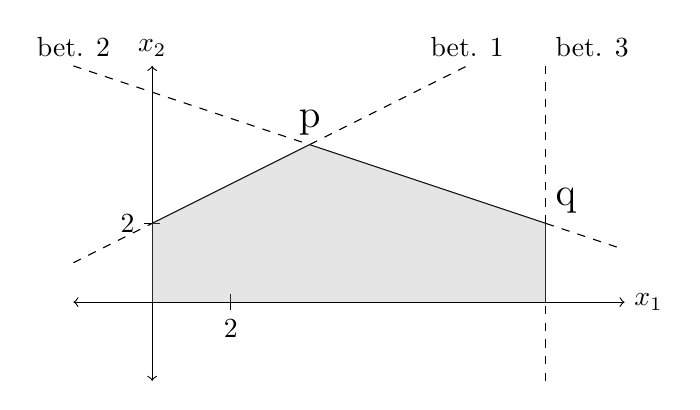
\begin{tikzpicture}
  %laver Grid. godt til når koordinater skal redigeres
  	%\draw[thin,gray!40] (-3,-1) grid (6,3); 
  %x-aksen
  	\draw[<->] (-1,0)--(6,0) node[right]{$x_1$};
  	%\draw[->,red] (2.5,0) -- (2.5,0.5);
  %y-aksen
  	\draw[<->] (0,-1)--(0,3) node[above]{$x_2$};
  	%\draw[->,red] (0,0.5) -- (0.5,0.5);
  	
  %akse-markeringer
  	%\node[left] (xakse) at (0,1) {2};
  	\draw[] (-0.1,1) -- (0.1,1) node[pos=0,left] {2};
  	\draw[] (1,-0.1) -- (1,0.1) node[pos=0,below] {2};
  	
  %ligning 1
	\draw[domain=-1:0,variable=\x,dashed] 	plot({\x},{0.5*\x+1});
	\draw[domain=0:2,variable=\x] 			plot({\x},{0.5*\x+1});
	\draw[domain=2:4,variable=\x,dashed] 	plot({\x},{0.5*\x+1}) node[above] {bet. 1};
  	%\draw[->,red] (1,1.5) -- (1.224,1.05);
	
  %ligning 2
  	\draw[domain=-1:2,variable=\x,dashed] 	plot({\x},{-(1/3)*\x+8/3}) node[above] at (-1,3) {bet. 2} ;
	\draw[domain=2:5,variable=\x] 			plot({\x},{-(1/3)*\x+8/3});
	\draw[domain=5:6,variable=\x,dashed] 	plot({\x},{-(1/3)*\x+8/3});
	%\draw[->,red] (3.5,1.5) -- (3.34,1.026);

  %ligning 3
  	\draw[domain=-1:0,variable=\y,dashed] 	plot({5},{\y});
	\draw[domain=0:1,variable=\y] 			plot({5},{\y});
	\draw[domain=1:3,variable=\y,dashed] 	plot({5},{\y}) node[above right] {bet. 3};
	%\draw[->,red] (5,0.5) -- (4.5,0.5);

  %nodes med navne på punkter
	\node[above] (p) at (2,2) {\Large p};
	\node[above right] (q) at (5,1) {\Large q};

  %løsningsmængden skraveret
	\fill[gray!80,nearly transparent] (0,0) -- (0,1) -- (2,2) -- (5,1) --(5,0) --  cycle;
\end{tikzpicture}
	\captionof{figure}{Løsningsmængde med naboløsninger $p$ og $q$.}
	\label{fig:nabo}
	\end{center}
	
\label{eks:nabo}
\end{eks}

%ved ikke: Må et afsnit slutte med et eksempel?




